\documentclass[10pt]{article}
\usepackage{icmlko}

\icmlmeta{IP 파운데이션 월드모델}{313}{빌리는 것은 검색이지 달력이 아니다}{도서의 빌림을 아홉 축으로 갈랐다 --- 검색 셋이 전부고 달력 여섯은 정확히 0 이다}

\begin{document}

\twocolumn[
\icmlheader

\begin{abstract}
노트 312가 도서의 빌림을 $t{=}{-}3.79$ 로 굳혔다. 잡음이 작은 자(F6, 짝SE
0.030)가 생겼으니 이제 \textbf{아홉 축을 갈} 수 있다. 갈랐다. \textbf{검색
셋이 전부다} --- \texttt{trend\_*} 셋을 통째로 끄면 $+$0.1132($t{=}{-}3.48$,
문턱 넘음)이고 \textbf{달력 여섯을 통째로 끄면 $-$0.0051}($t{=}{+}0.55$)로
\textbf{0 이다} --- 오히려 끄는 쪽이 아주 살짝 낫다. 낱개로는 아무것도 문턱을
못 넘는다(제일 큰 \texttt{trend\_level} 이 $+$0.0681 · $t{=}{-}2.35$).
그리고 낱개 합 $+$0.0930 이 셋 묶음 $+$0.1132 보다 \textbf{작다} --- 셋이
\textbf{함께} 쓰인다. \textbf{그러니 이 실험실이 실제로 보인 전이는 한
문장이다}: \emph{오픈 이전 검색 관심이 성과로 바뀌는 방식}을 웹툰 · 애니 ·
게임 · 모바일에서 배워 \textbf{도서 행에 그대로 적용한다.} 도서 자신에서는
그 축이 라벨과 아무 관계가 없다(그래서 ``안 오른다''로 판정됐다). 그런데
남이 정한 대응을 받으면 $\rho$ 0.31 중 \textbf{0.11}이 거기서 나온다.
\textbf{그리고 오래 끌어 온 달력 갈래는 이 자리에서도 빈손이다} --- 달력은
빌려 주지도 빌려 오지도 않는다.
\end{abstract}
]

\section{이제 갈 수 있다}

노트 303이 도서의 빌림을 처음 재고, 노트 312가 자를 바꿔 $t{=}{-}3.79$ 로
굳혔다. \textbf{짝SE 가 0.030 이면 0.03 짜리 차이를 볼 수 있다} --- 아홉
축을 하나씩 끌 수 있다는 뜻이다. F18(짝SE 0.048)로는 못 했다.

\paragraph{도서가 빌리는 아홉} \texttt{trend\_level} · \texttt{momentum} ·
\texttt{volatility}(네이버 검색, 오픈 이전 12주) $+$ \texttt{cal\_dow\_sin} ·
\texttt{dow\_cos} · \texttt{weekend} · \texttt{month\_sin} ·
\texttt{month\_cos} · \texttt{holiday\_gap}(달력).

\section{검색 셋이 전부다}

\begin{figure*}[t]
\centering
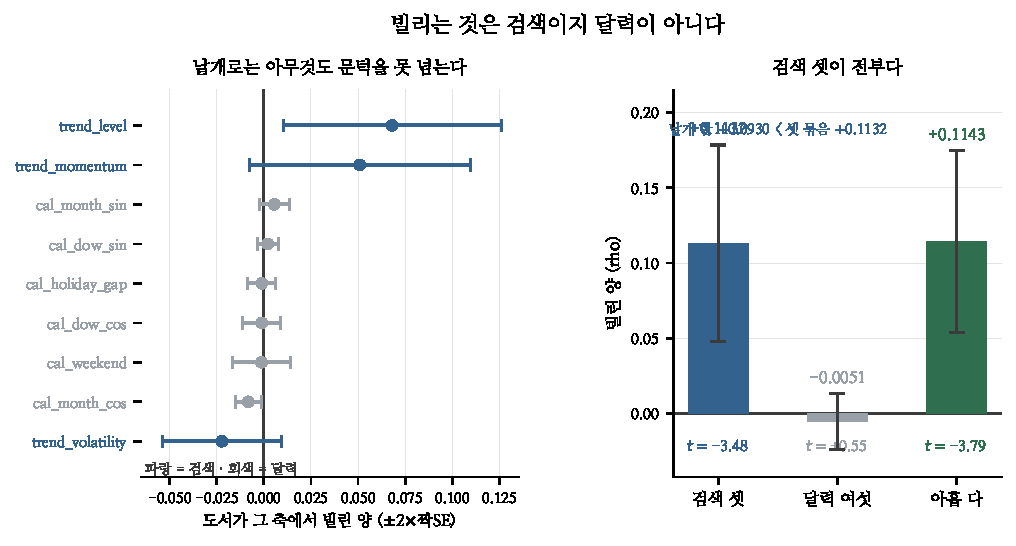
\includegraphics[width=\textwidth]{figs/which.pdf}
\caption{왼쪽 --- 축 하나씩 껐을 때 도서가 잃는 양($\pm$2$\times$짝SE,
부트스트랩 400). 오른쪽 --- 계열로 묶은 것.}
\end{figure*}

\begin{center}\small
\begin{tabular}{lrrr}
\hline
& 빌림 & 짝SE & $t$ \\
\hline
\textbf{검색 셋} & \textbf{$+$0.1132} & 0.0326 & \textbf{$-$3.48} \\
달력 여섯 & $-$0.0051 & 0.0093 & $+$0.55 \\
\hline
아홉 다 & $+$0.1143 & 0.0302 & $-$3.79 \\
\hline
\end{tabular}
\end{center}

\textbf{달력 여섯이 0 이다.} 그것도 ``못 잰다''가 아니라 짝SE 0.0093 에
$-$0.0051 --- \textbf{$\pm$0.019 안에 있다.} 오히려 부호가 음수라 끄는 쪽이
살짝 낫다.

\begin{center}\footnotesize
\begin{tabular}{lrrr}
\hline
축 & 빌림 & 짝SE & $t$ \\
\hline
\texttt{trend\_level} & $+$0.0681 & 0.0289 & $-$2.35 \\
\texttt{trend\_momentum} & $+$0.0509 & 0.0293 & $-$1.74 \\
\texttt{cal\_month\_sin} & $+$0.0056 & 0.0040 & $-$1.38 \\
\texttt{cal\_dow\_sin} & $+$0.0021 & 0.0028 & $-$0.77 \\
\texttt{cal\_holiday\_gap} & $-$0.0011 & 0.0037 & $+$0.29 \\
\texttt{cal\_dow\_cos} & $-$0.0011 & 0.0050 & $+$0.21 \\
\texttt{cal\_weekend} & $-$0.0012 & 0.0077 & $+$0.15 \\
\texttt{cal\_month\_cos} & $-$0.0082 & 0.0035 & $+$2.37 \\
\texttt{trend\_volatility} & $-$0.0222 & 0.0157 & $+$1.41 \\
\hline
\end{tabular}
\end{center}

\paragraph{낱개로는 아무것도 못 넘는다} 제일 큰 \texttt{trend\_level} 이
$t{=}{-}2.35$ 다. 그리고 \textbf{낱개 합 $+$0.0930 이 셋 묶음 $+$0.1132 보다
작다} --- \textbf{셋이 함께 쓰인다}(수준 · 기울기 · 변동을 같이 봐야 뜻이
생긴다). \texttt{trend\_volatility} 는 혼자 끄면 오히려 도움이 되는데
($-$0.0222) 셋 중 하나로는 값을 낸다.

\section{그래서 전이가 한 문장이 된다}

\begin{center}\small
\begin{tabular}{l}
\hline
\emph{오픈 이전 검색 관심이 성과로 바뀌는 방식}을 \\
웹툰 · 애니 · 게임 · 모바일에서 배워 \\
\textbf{도서 행에 그대로 적용한다} \\
\hline
\end{tabular}
\end{center}

도서 자신에서는 그 축이 라벨과 아무 관계가 없다 --- 그래서 노트 300의 검사
③ 이 ``안 오른다''로 판정했다. 학습 80행으로는 ``검색이 많으면 잘 팔린다''를
못 배운다. \textbf{그런데 웹툰 2,106행 · 애니 1,467행이 정한 대응을 받으면}
도서 유보 $\rho$ 0.3108 중 \textbf{0.1132}가 거기서 나온다.

\paragraph{그리고 노트 310이 설명된다} 노트 310이 ``빌린 양은 그 축이 그
도메인에서 새로운가로 정해진다''($\rho{=}{+}0.803$)를 냈다. 그 ``새롭다''
개수를 \emph{검색 축만} 세면 웹툰 3 · 애니 3(둘 다 세 축 다) · 모바일 3 ·
게임 3 이고 세계애니 · 만화는 \textbf{검색 덮음이 0\%} 라 셀 것이 없다.
LOO 상위가 웹툰 · 애니였던 것과 맞는다.

\paragraph{다만 만화가 안 맞는다} LOO 에서 만화가 셋째였다($-$0.0491,
$t{=}{-}1.93$)는데 만화는 검색 덮음이 0\% 다 --- 빌려 줄 검색 구조가 없다.
문턱 아래라 크게 안 읽지만 \textbf{열어 둔다.}

\section{달력은 이 자리에서도 빈손이다}

오래 열린 갈래가 ``달력이 왜 트리에서만 되는지''인데, 노트 311이 다섯째
설명(나무만 빌릴 수 있다)을 죽였고 이 노트가 하나를 더한다 ---
\textbf{달력은 빌려 주지도 빌려 오지도 않는다.}

\begin{center}\footnotesize
\begin{tabular}{ll}
\hline
달력에 대해 아는 것 & \\
\hline
전 도메인 100\% 덮음 & 노트 306 \\
열 도메인 중 셋에서만 ``새롭다'' & 노트 300 \\
도서가 달력에서 빌리는 양 & \textbf{$-$0.0051} (이 노트) \\
\hline
\end{tabular}
\end{center}

\textbf{공짜로 얻어서 전부에게 붙였는데 옮기지도 못한다.} 달력이 어디서
일하는지(웹툰 · 애니 안에서)는 여전히 관측이다.

\paragraph{남은 것}
\begin{center}\small
\begin{tabular}{ll}
\hline
갈래 & 왜 \\
\hline
만화가 왜 셋째였나 & 검색 덮음 0\% 인데 \\
검색 덮음을 도서에 & 지금 89\% --- 100 이면 더 빌리나 \\
펀딩도 검색인가 & 검색 덮음 100\% 다 \\
달력을 떼면 & 판이 어떻게 되나 \\
\hline
\end{tabular}
\end{center}

\paragraph{규약} \textbf{자가 좋아지면 예전에 못 물었던 것을 물어라.}
``도서가 무엇을 빌리나''는 노트 303 때도 물을 수 있었지만 F18 의 짝SE
0.048 로는 0.005 짜리 달력 효과와 0.11 짜리 검색 효과를 못 갈랐다.
\textbf{자를 바꾸는 것이 표본을 늘리는 것과 같은 일을 한다}(노트 311).
그리고 \textbf{묶어서 문턱을 넘은 것을 낱개로 다시 물어라} --- 셋 다 낱개로는
못 넘는데 묶으면 넘고, 합보다 묶음이 크다. \textbf{그것이 ``함께 쓰인다''의
증거다.}

\end{document}
